
\documentclass[a4paper,12pt]{article}
\usepackage[T1]{fontenc}
\usepackage[utf8]{inputenc}
\usepackage[english]{babel}
%% PAGE LAYOUT
\usepackage[a4paper,hmargin=1.2in,top=2.5in,bottom=1in,marginpar=0in]{geometry}
%% FONT
\usepackage{helvet}
% set default document font to sans serif
\renewcommand{\familydefault}{\sfdefault}
%% TikZ (for placing stuff on the page, e.g., header art)
\usepackage{tikz}
\usepackage{graphicx}
%%
%\usepackage{paralist}
\usepackage{ragged2e}
\usepackage{array}
  \newcolumntype{L}[1]{>{\RaggedRight\let\newline\\\arraybackslash\hspace{0pt}}m{#1}}
  \newcolumntype{C}[1]{>{\Centering\let\newline\\\arraybackslash\hspace{0pt}}m{#1}}
  \newcolumntype{R}[1]{>{\RaggedLeft\let\newline\\\arraybackslash\hspace{0pt}}m{#1}}
\usepackage{booktabs}
\usepackage{csquotes}

% no page numbers
\pagestyle{empty}

\begin{document}
% Suppress paragraph indentation
\setlength{\parindent}{0in}
\setlength{\parskip}{1ex plus 0.5ex minus 0.2ex}


\begin{tikzpicture}[remember picture, overlay]
  % header artwork
  \node at (current page.north west) [anchor=north west, inner sep=0pt] {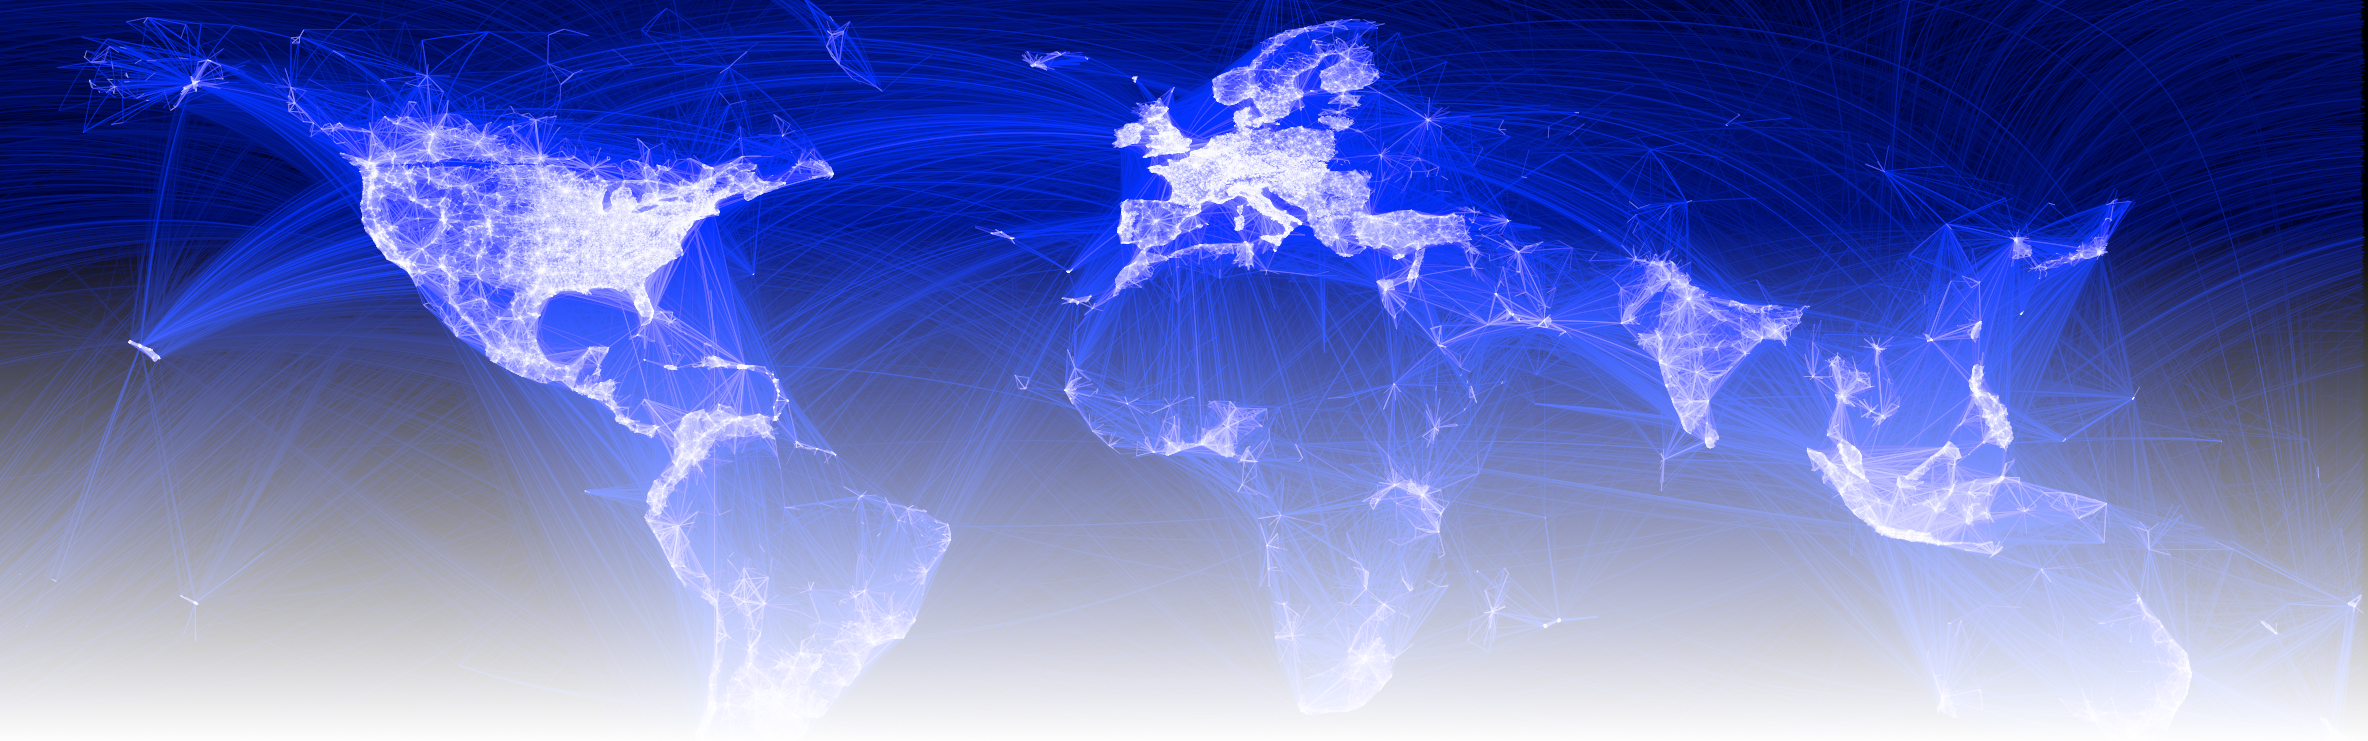
\includegraphics[width=210mm]{socialgraph}};
  % text on top of header art
  \node at (current page.north east) [anchor=north east, color=white, font=\rmfamily\Large\bfseries, xshift=-0.2in, yshift=-0.1in, align=right] {Mon Sep 19--Thu Sep 22, 2pm\\at Ångströmlab.};
  % https://www.facebook.com/notes/facebook-engineering/visualizing-friendships/469716398919
  % reference to Butler in footer
  \node at (current page.south west) [anchor=south west, inner sep=0pt, xshift=1.2in, yshift=0.8in, font=\footnotesize, align=left] {Header art adapted from Paul Butler, Facebook, 2010. \enquote{Visualising friendships}.\\Butler used R to visualise the dataset.};
  % UU logo in bottom right corner
  \node at (current page.south east) [anchor=south east, inner sep=0pt, xshift=-0.2in, yshift=0.1in] {\includegraphics{UU_logo_sv_30}};
\end{tikzpicture}



\section*{R for physical scientists}

% R is one of the fastest growing programming languages for scientific data analysis, statistics and visualisation. R is free and open source software (FOSS).

R is a freely available, open source programming language for scientific data analysis, statistics and visualisation. It has a vibrant community, and is one of the fastest growing programming languages. R is a powerful alternative to MATLAB for researchers in physics and chemistry.

\textbf{Aim of the course:} To get you up and running with using R for typical data analysis and plotting tasks. At the end of this short course you should be confident with importing data from common formats, organising and manipulating data, and visualisation.

%using R with your own data. At the end of this short course you should be able to read your datasets into R, manipulate and shape the data into an appropriate format, and visualise it.
% suggested addition:
% - share your data, plots with others

% could be more specific here perhaps -Matt.
% for example
\textbf{Target group:} Graduate students in science and engineering who are interested in, learning to write simple programs to really speed up routine data analysis, making better graphs, thinking about old problems in new ways, learning a versatile programming language, and so on!\\

%%Graduate students in science and engineering who are willing to take the training wheels off! (The training wheels being Excel, Origin and their ilk).

%who want their work to be less dependent on proprietary software and who would like their research work to be more reproducible and easily shareable...

%\textbf{Course content:}
%\begin{inparaitem}%
%  \item Ingesting and manipulating data (vectors, functions, matrices, lists, dataframes).
%  \item Visualising data using the grammar of graphics (ggplot2).
%\end{inparaitem}

\begin{center}
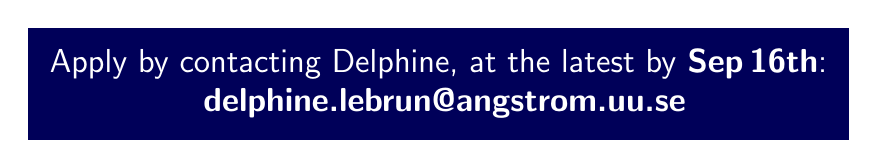
\begin{tikzpicture}
  \node  [color=white, font=\large, fill= black!65!blue, align=center,inner sep=8.0pt] {Apply by contacting Delphine, at the latest by \textbf{Sep\,16th}: \\  \textbf{ delphine.lebrun@angstrom.uu.se}};
\end{tikzpicture}

\end{center}


\subsection*{Schedule and content}

\textbf{Topics}: Basic R (objects, functions, etc), importing data (e.g., from Excel, plain text), making plots (\texttt{ggplot2}), manipulating data (incl. the \texttt{dplyr} package), writing readable code (\texttt{magrittr}), reporting (\LaTeX{} support, R Markdown) and more!

\begin{center}\small
\begin{tabular}{L{2.5cm}L{2.5cm}L{2.8cm}L{2.5cm}}\toprule
Mon 19th    & Tue 20th   & Wed 21th   & Thu 22nd   \\\midrule
\multicolumn{2}{c}{Mellanrummet}  & Beurlingrummet    & Mellanrummet \\
14:00--17:00    & 14:00--17:00     & 14:00--17:00       & 14:00--18:00 \\

\bottomrule
\end{tabular}
\end{center}


This course is organised by Delphine Lebrun, Taha Ahmed and Matt Lacey (Dept of Engineering Sciences and Dept of Chemistry--Ångström).


\end{document}


If you are interested, send your name and affiliation to \emph{Delphine Lebrun}, at the latest by Sep 16th.


\subsection*{Schedule and content}

\begin{center}\small
\begin{tabular}{L{2cm}L{2cm}L{2cm}L{2cm}}\toprule
Monday    & Tuesday    & Wednesday    & Thursday    \\\midrule
14--17    & 14--17     & 14--17       & 14--18 \\
          & the first serpentine, a twisting road to nowhere
                       & a very long and winding line
                                      & is this the last tortuous journey down a well-worn path?\\
\bottomrule
\end{tabular}
\end{center}


This course is organised by Delphine Lebrun, Taha Ahmed and Matt Lacey (Dept of Engineering Sciences, Solid state physics and Dept of Chemistry--Ångström).


\end{document}

